\chapter{Introducción}
\section{Antecedentes y motivación}
\indent Visión por computador es una disciplina que intenta emular las capacidades de la visión humana para identificar y clasificar diferentes objetos desde una imagen. Es un área de investigación muy amplia, que se entrelaza con diferentes campos de investigación en el ámbito de las ciencias de la computación y el desarrollo tecnológico. Tiene como desafío facilitar máquinas computacionales con capacidad de percepción humana, en otras palabras comprender el medio ambiente, tomar acciones, aprendizaje, y mejorar desempeño de acciones tomadas. Visión por computador intenta hacer una descripción del mundo que los seres humanos pueden observar, a través de imágenes para hacer una reconstrucción de sus principales propiedades.

\indent Hay en el último tiempo un constante desarrollo de nuevas técnicas y aparatos tecnológicos, que incorporan algoritmos empleados en visión por computador, en heterogéneos campos de aplicación. Se está experimentando algoritmos inteligentes en vehículos que permiten evitar obstáculos, reconocer peatones o viajar de un punto a otro sin la intervención de un conductor. En dispositivos audiovisuales, como cámaras fotográficas digitales, algoritmos de reconocimiento de figuras y rostros es una característica normal incluida en estos artefactos. Se utilizan además, las técnicas de análisis y reconocimiento de patrones en imágenes médicas, o clasificación de acciones humanas en cámaras de vigilancia, entre muchas otras aplicaciones.


\begin{figure}
\centering     %%% not \center
\subfigure[Evitar obstáculos]{\label{fig:Figure_A}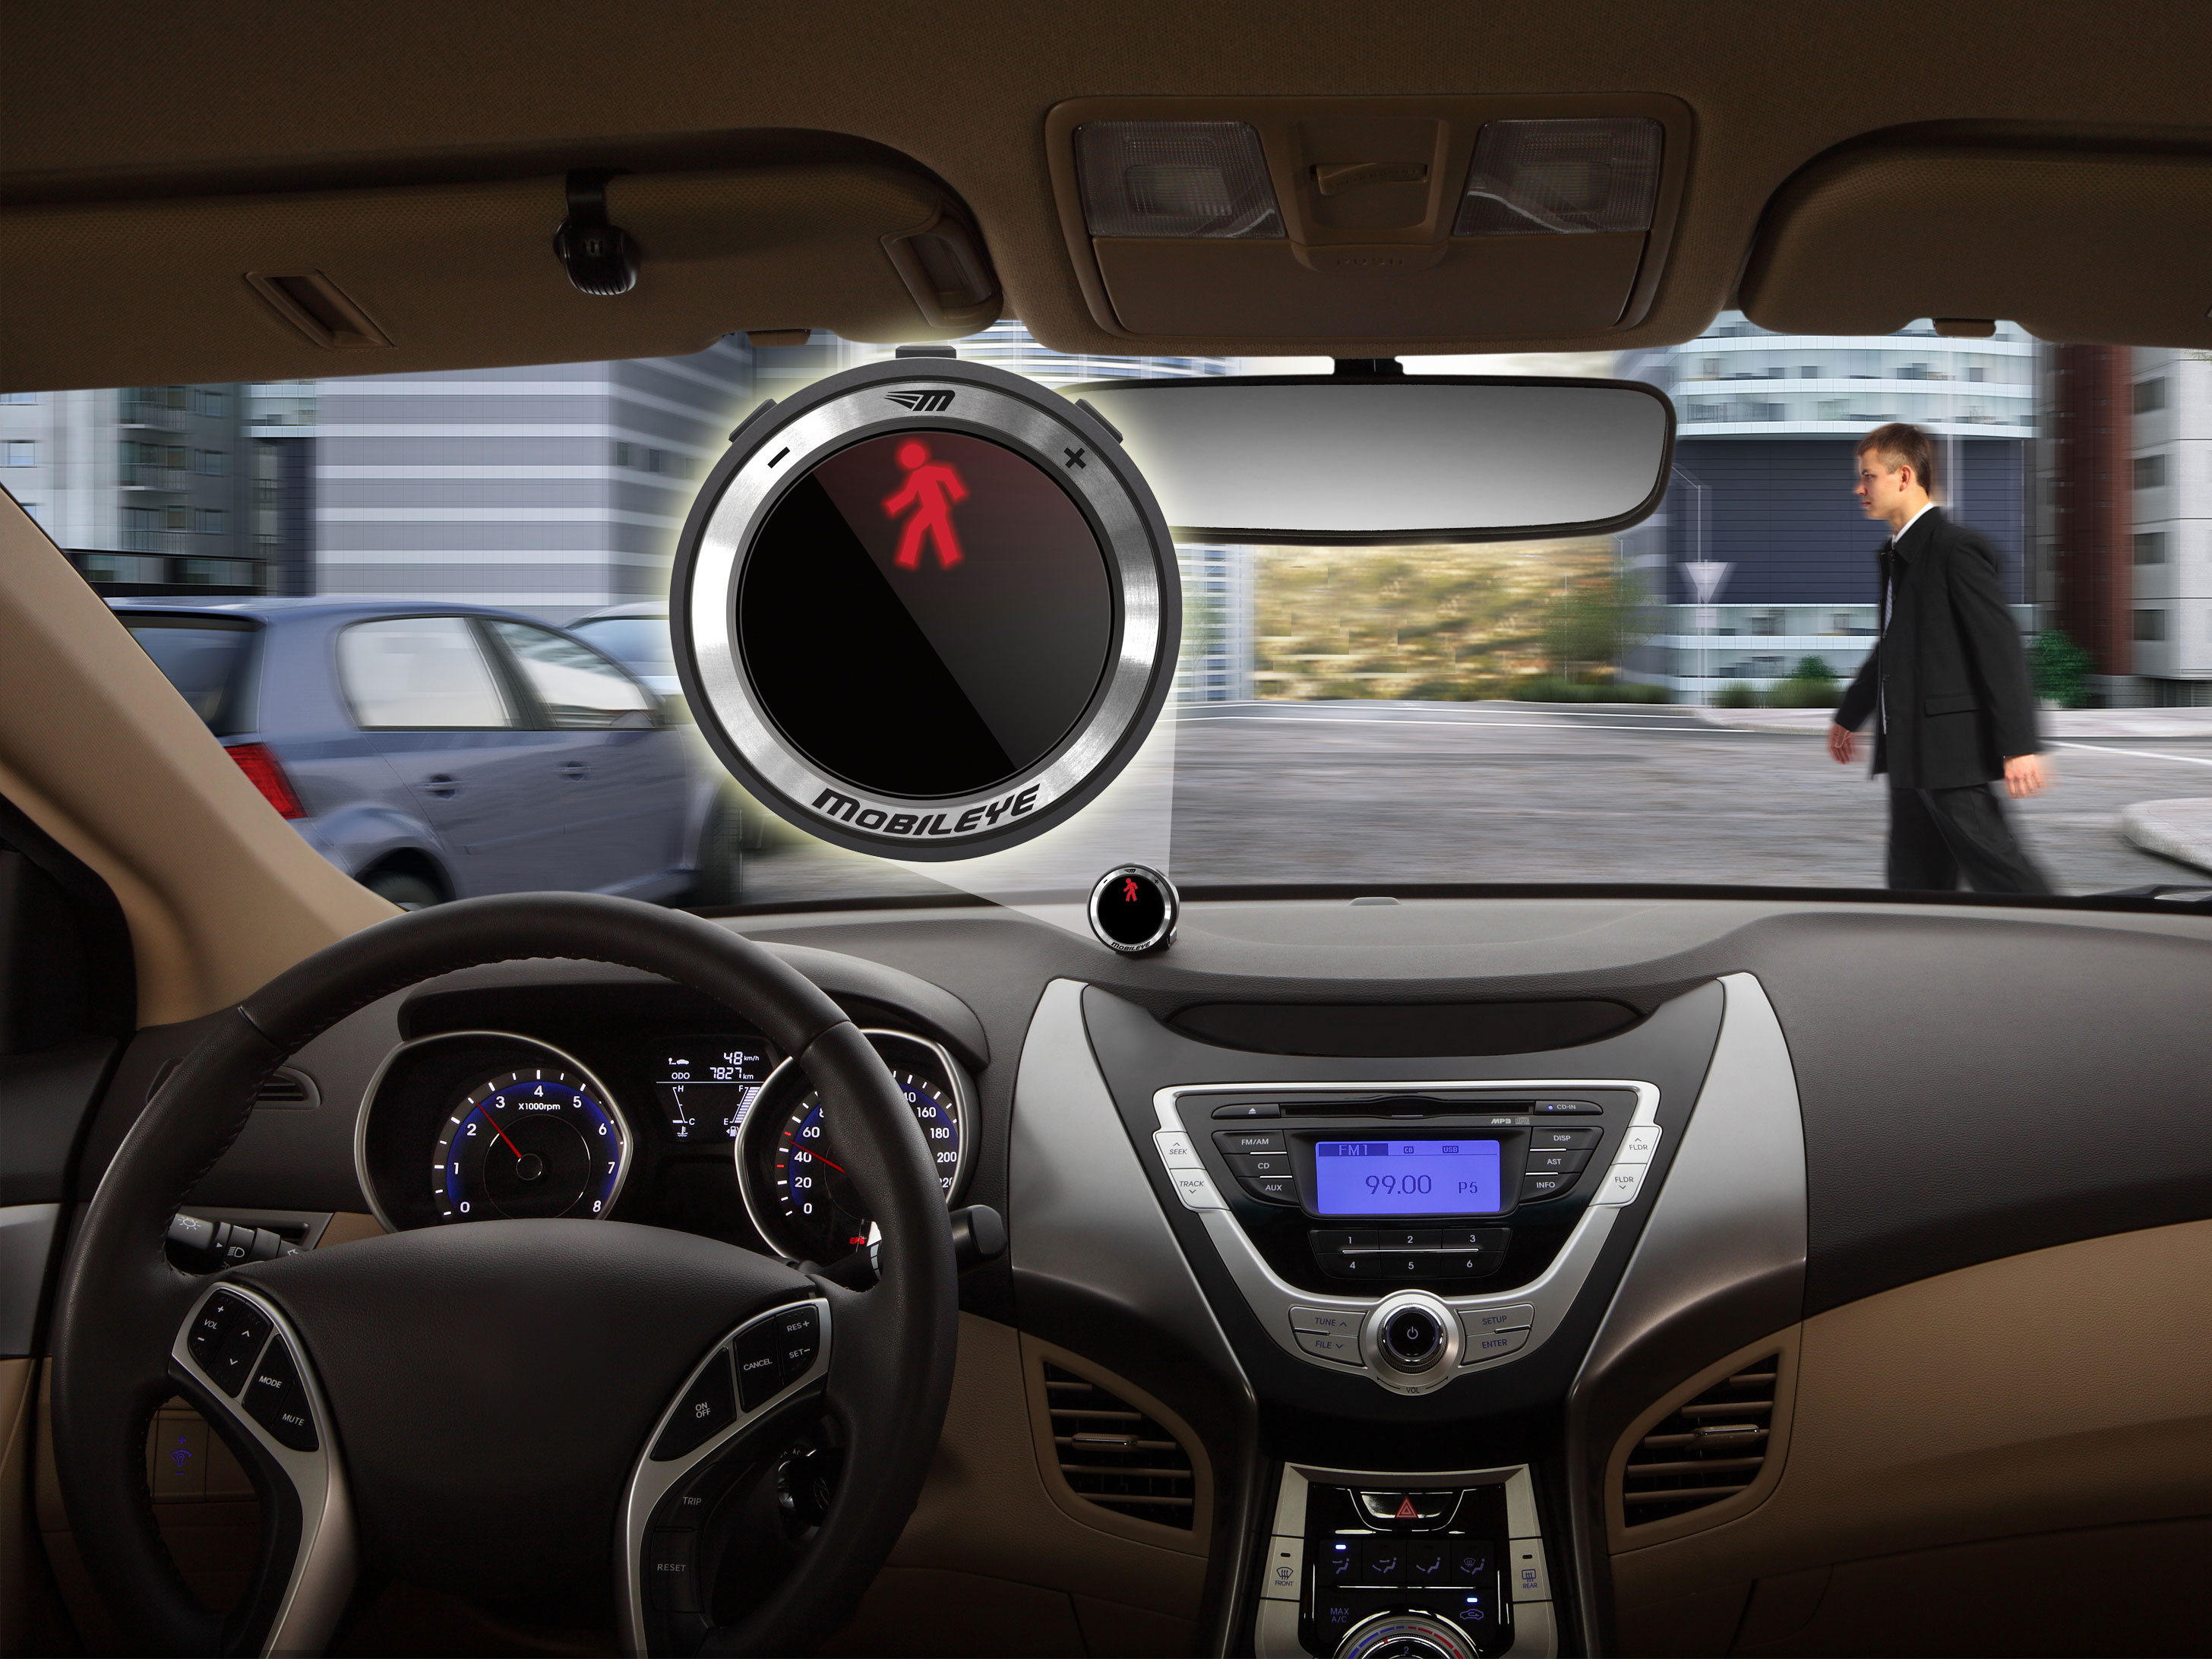
\includegraphics[width=50mm]{img/MobileEyemaster}}
\subfigure[Reconocimiento de vehículos]{\label{fig:Figure_B}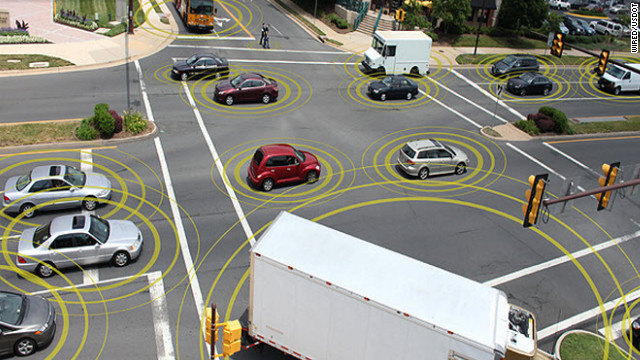
\includegraphics[width=50mm]{img/self-driving-cars}}
\subfigure[Reconocimiento de peatones]{\label{fig:Figure_C}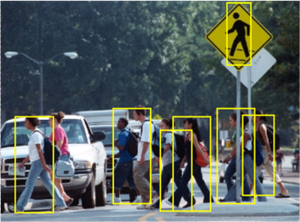
\includegraphics[width=50mm]{img/crossing}}
\subfigure[Experimentación con vehículos autónomos \tiny{(Figure courtesy Google \copyright )}]{\label{fig:Figure_D}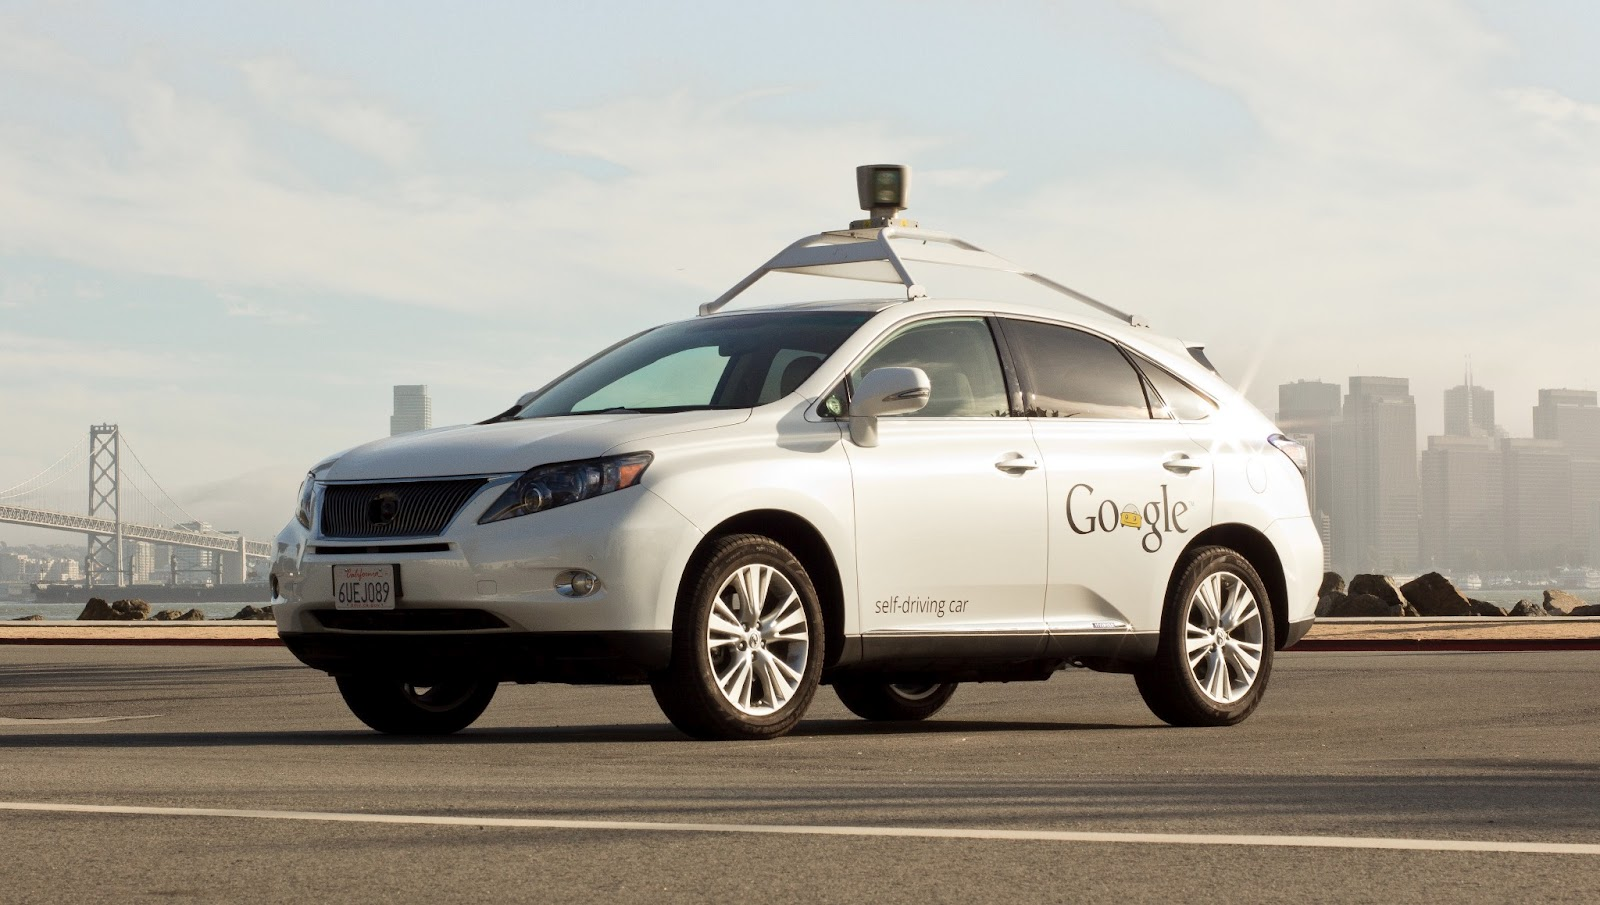
\includegraphics[width=50mm]{img/Google500KmilesLexus}}
\subfigure[Reconocimiento de caras \tiny{(http://www.netmechanic.co.za/ \copyright)}]{\label{fig:Figure_E}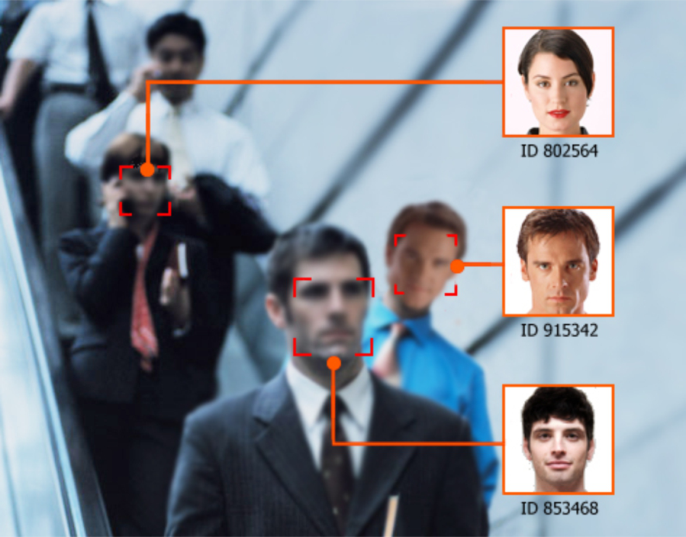
\includegraphics[width=50mm]{img/face_recognition_technology}}
\caption[Aplicaciones en visión por computador]{Imagenes de aplicaciones en visión por computador }
\label{fig:aplicaciones_vision_por_computador}
\end{figure}


\indent Las diferentes etapas de la cadena de procesamiento en visión por computador constituyen un conjunto extenso de técnicas, algoritmos y métodos provenientes, entre otros, del mundo de procesamiento digital de imágenes y clasificación del área de máquinas de aprendizaje computacional. En cada una de estas etapas además, se emplean diferentes aproximaciones para dar solución al problema que se intenta resolver. La figura \ref{fig:etapas_vision_computador}, es un diagrama general de las distintas etapas que intervienen en un sistema de visión por computador. Una primera etapa consiste en la adquisición de secuencia de imágenes. Las diferentes imágenes del campo de aplicación que se quiere estudiar, son obtenidas mediante algún dispositivo sensor (cámara de vídeo) que transforma una escena del mundo real en una señal electrónica. Las señales son muestreadas y discretizadas para ser convertidas en una matriz de números que representan la escena en un conjunto de imágenes digitalizadas. La etapa de pre-procesamiento se refiere principalmente al mejoramiento de la entrada por medio de técnicas de procesamiento digital de imágenes. Se aplican métodos en el dominio espacial (transformaciones, filtros espaciales, extensión de contraste, procesamiento y ecualización de histogramas, entre otros) y en el dominio de la frecuencia (técnicas basadas en modificar la transformada de \textit{Fourier} de una imagen) para acondicionar las imágenes que permitan resaltar alguna propiedad que requiera la aplicación específica. El proceso de segmentación es una etapa de subdivisión de objetos en una imagen. Se agrupan componentes de una imagen en elementos que tengan alguna característica propia, como forma, color o distribución estadística del color. Un procedimiento similar complementario a la segmentación, es la sustracción del fondo de imagen en una secuencia, esta consiste en modelar el fondo de imagen y sustraer mediante diferentes técnicas los objetos que están sobre ese fondo modelado. La etapa de extracción de características transforma las imágenes de entrada en una representación de elementos característicos agrupados en un vector de propiedades de la imagen o vector característico. Estos vectores sirven de base en la etapa de clasificación o reconocimiento de patrones. 



\begin{figure}[h!]
  \centering
      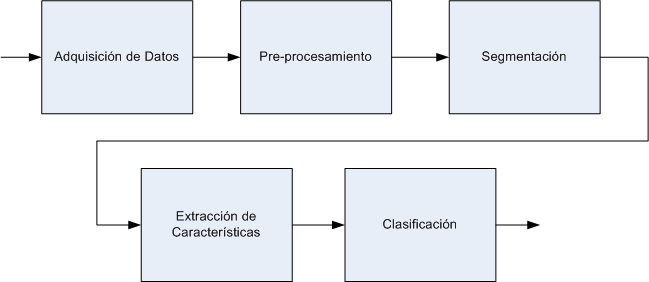
\includegraphics[scale=0.5]{img/generic_block_diagram_computer_vision}
  \caption[Diagrama de bloques etapas visión por computador]{Diagrama de bloques genérico de las diferentes etapas en visión por computador}
\label{fig:etapas_vision_computador}
\end{figure}

\indent El reconocimiento y clasificación de actividades humanas es una de las tareas más complejas dentro del quehacer de visión por computador, la cual tiene un desarrollo constante dentro de los grupos dedicados a la investigación dentro de este campo. Existe un desafío permanente para desarrollar nuevas técnicas y algoritmos que mejoren los métodos de detección y clasificación de siluetas (``\textit{foreground}'') desde un segundo plano (``\textit{background}'') en una secuencia de imágenes, en diferentes condiciones de iluminación y sombras. Se emplean por ejemplo, algoritmos que construyen un modelo estadístico de los ``píxeles'' de la imagen de fondo, o algoritmos que comparan distribuciones (histogramas) para hacer el seguimiento de objetos en una secuencia de video (``\textit{mean shift tracking}''). 

\indent Se requiere un conjunto preestablecido de imágenes o vídeos, que posibiliten evaluación y comparación de las técnicas y métodos utilizados en segmentación, clasificación y reconocimiento de actividades humanas. En este contexto, existe una variedad de conjuntos de datos (``\textit{datasets}'') disponibles en la comunidad, para ser usados como parte del proceso de evaluación y comparación de algoritmos. Estas base de datos públicas, se componen de imágenes y acciones en secuencia, tomadas desde el mundo real en diferentes ángulos de observación, condiciones ambientales e iluminación.

\indent Los investigadores requieren alguna referencia que les permita evaluar y comparar sus modelos. Deben asegurar que el modelo desarrollado cumple con los objetivos propuesto originalmente. En este ambiente surgen diferentes metodologías de evaluación de modelos, así como los conjuntos de datos que permiten emular un medio ambiente sobre el cual los algoritmos pueden ser ejecutados. 



\indent La finalidad de este trabajo de tesis, consiste en una primera etapa, implementar una plataforma de software que permita, incorporar y evaluar nuevos algoritmos de visión por computador. Es un sistema prototipo de software que pretende establecer una base estándar de evaluación de desempeño de distintos tipos de algoritmos, relevantes en el desarrollo del campo de visión por computador. Este sistema de software viene para ayudar a reducir los tiempos de desarrollos de nuevos algoritmos y evaluar cambios de comportamiento de pequeñas modificaciones en algoritmos desarrollados. Proporciona una infraestructura base para desarrollar y posteriormente evaluar desempeño de nuevos software en visión por computador. Una segunda parte se propone consolidar las métricas de evaluación más utilizadas del campo de clasificación, en una herramienta de software única. Se busca de esta manera, obtener una métrica final de evaluación. El escenario de evaluación utilizado es MuHAVI \cite{singh_muhavi_2010}, un conjunto de datos públicos que dispone diferentes acciones y condiciones orientado a la detección de acciones humanas.


\section{Descripción del problema}
\indent Este trabajo plantea la utilización de un conjunto de datos de reconocimiento de acciones humana “MuHAVI” \cite{singh_muhavi_2010} (``\textit{Multicamera Human Action Video dataset}''), como soporte de comparación y evaluación de rendimiento, de varios algoritmos de sustracción de imágenes de fondo (\textit{Background Subtraction}).  Para esto se propone consolidar un conjunto de métricas de evaluación, utilizadas en clasificación, en una herramienta de software que permita evaluar y comparar las siluetas resultantes de estos algoritmos, con una versión anotada de siluetas que dispone la versión mejorada del conjunto de datos MuHAVI-MAS (``\textit{Manually Annotated Silhouette}'') . 


\indent Se busca adaptar el algoritmo desarrollado por Zezhi Chen \cite{chen_vehicle_2012}, propuesto inicialmente para localización, clasificación y seguimiento de vehículos, y otras versiones equivalentes de sustracción de fondo, en un único sistema de software que incorpore estas diferentes aproximaciones y generar un conjunto total de siluetas de las diferentes secuencias en MuHAVI para evaluar el rendimiento final de cada algoritmo.



\section{Solución propuesta}

\indent Se proyecta desarrollar un sistema de software, basado en un modelo orientado a objetos, que permita evaluar algoritmos de detección y clasificación de actividades humanas. Este software además, implementa e incorpora diferentes versiones de algoritmos de sustracción de fondos, para proporcionar un conjunto de siluetas como resultado final. Facilitando el proceso de evaluación de la herramienta de software principal.

\indent El código implementado para esta solución estará constituido por una biblioteca de clases en C++, que permitiría re-usar su código para diferentes tipos de algoritmos de detección de actividades humanas.

\indent Este trabajo considera varios artefactos de software como entrega final; un sistema de evaluación de algoritmos, un ``framework'' de software que incorpore los diferentes algoritmos de sustracción de fondo, y un conjunto de siluetas necesarias para los algoritmos implementados y otras versiones de estos.

\indent El resultado será un prototipo de software que puede constituir la base para el desarrollo de una plataforma de evaluación de algoritmos empleados en visión por computador.



\section{Objetivos y alcances del proyecto} 
\subsection{Objetivo general}

\indent Implementar un sistema prototipo de software, que incorpore algoritmos de sustracción de fondo empleados en visión por computador, y desarrollar una herramienta de software de evaluación de desempeño para los algoritmos implementados, con el propósito de generar automáticamente siluetas desde conjunto de datos de reconocimiento de acciones humana usando el algoritmo de mejor rendimiento.

\subsection{Objetivos específicos}

\begin{itemize}
\item Implementar el algoritmo de sustracción de fondo propuesto por Zezhi Chen\cite{chen_vehicle_2012} en un programa ejecutable desarrollado en un lenguaje de programación C++ orientados a objeto.
\item Desarrollar un sistema de software base que incorpore otros algoritmos de sustracción de fondo.
\item Implementar una herramienta de software que consolide las métricas más utilizadas en sistemas de clasificación.
\item Evaluar las siluetas resultantes de los distintos algoritmos ejecutados sobre MuHAVI.
\item Generar curvas comparativas del desempeño de los algoritmos.
\item Generar y publicar el conjunto total de siluetas resultantes del algoritmo con mejor desempeño para de todas las secuencias del conjunto de datos MuHAVI 
\end{itemize}


\subsection{Alcances} 

Este trabajo tesis considera varios artefactos como entrega final; desarrollo de un software prototipo que incorpora algoritmos de sustracción de fondo, identificación de métricas de evaluación de calidad, implementación de un programa que evalúa siluetas obtenidas por los distintos algoritmos, un conjunto de siluetas producidas automáticamente, evaluación de desempeño del conjunto de algoritmos de detección de fondo incluidos en el sistema de software prototipo.
El resultado será un prototipo que puede constituir la base para el desarrollo de un ``framework'' de software para evaluación de otros algoritmos de usados en la detección de actividades humanas.


\section{Metodologías y herramientas utilizadas} 

\indent La metodología a utilizar en el desarrollo de este trabajo de tesis, se apoyará en una etapa de investigación, implementación y verificación de resultados. Esta metodología estará basada en las actividades del método científico

\begin{itemize}
\item Identificación del problema. Existe un nuevo método de detección, seguimiento y clasificación de vehículos en autopistas urbanas que podría adaptarse para ser usado en detección de actividades humanas sobre una base de datos denominada MuHAVI.

\item Planteamiento de una hipótesis. Los algoritmos que componen el método Z Chen \cite{chen_vehicle_2012} pueden ser adaptados e implementados para ser usados sobre MuHAVI en la detección de actividades humanas.

\item Revisión de la literatura: Esta etapa consiste en hacer una revisión de las distintas publicaciones que dieron origen a la mejora de este método propuesto por Z Chen \cite{chen_vehicle_2012}. Además, revisar los actuales trabajos de clasificación basado en redes neuronales que permitan reconocimiento de actividades humanas.

\item Implementación del modelo: Se basa en la implementación de los algoritmos de este método en clases C++ basados en el framework de visión por computador ``OpenCV".

\item Etapa de validación y verificación certifica que la implementación realice detección de siluetas y posterior clasificación de estas. Es en esta etapa donde se hará un uso intensivo del software implementado para hacer una clasificación total de MuHAVI.

\item Análisis de resultados y conclusiones, los resultados obtenidos en la etapa anterior son contrastados y comparados para obtener conclusiones sobre el método implementado.
\end{itemize}

\subsubsection{Herramientas de desarrollo}

\begin{itemize}
\item Sistema operativo Linux Ubuntu 12.04
\item Biblioteca de maquinas de aprendizaje y visión por computador OpenCV versión 2.4.4 (``Open Source Computer Vision Library")
\item Compilador GNU C++
\item Sistema de control de versiones "GIT"
\item CMake.
\end{itemize}

\subsubsection{Ambiente de desarrollo}

\indent Es proyecto será realizado en dependencias particulares, se dispondrá de un equipo computacional para hacer el desarrollo de esta aplicación de software.





\section{Resultados obtenidos}

\textcolor{red}{Falta definir los resultados obtenidos}

\section{Organización del documento}

El primer capítulo de este trabajo de titulación se presenta el proyecto a desarrollar, se menciona el alcance, objetivo general, y lo objetivos específicos necesarios para lograr el objetivo general. Se detalla las herramientas necesarias para construir el proyecto, finalmente se hace una breve descripción de la solución propuesta. En segundo capítulo se hace una revisión bibliográfica de los principales temas abordados en la tesis. Se detalla el estado actual de los métodos de sustracción de fondo en la comunidad de investigación en visión por computador, especialmente en los métodos de modelado estadístico. Se mencionan las métricas más utilizadas para evaluar segmentación de imágenes y clasificación de actividades, también se hace una breve mención de los distintos conjunto de datos construidos especialmente para evaluación de algoritmos de detección de actividades. El tercer capítulo se dedica exclusivamente a describir los algoritmos implementados en este trabajo de tesis, se detalla el algoritmo de sustracción de fondo usando mixtura de componentes Gaussianas. El cuarto capítulo se dedica a mencionar las herramientas, los criterios y las decisiones para llevar a cabo este trabajo de tesis. Se describe también a nivel de bloques las distintas implementaciones de software realizadas, se presentan diagramas UML de paquetes y clases de los sistemas implementados. El quinto capítulo, se detalla el resultado de las experimentaciones, y sus análisis, se muestran también las curvas características de resultados. Finalmente el capítulo de las conclusiones, proporciona una idea del resultado general, se hacen las comparaciones de los diferentes algoritmos y se indican los posibles trabajos futuros que se podrían abordar a partir de este trabajo.



